\chapter{Introduction}

Language modelling has undergone a dramatic transformation in recent years. In 2021, the release of GPT-3, a language model with \textbf{175 billion parameters}, marked a significant milestone for the field of natural language processing (NLP). GPT-3 set a new standard for performance on a wide range of language understanding tasks, in many cases achieving or surpassing human-level capabilities \citep{brown2020gpt3}. At the time, its unprecedented scale drew comparisons to the 86 billion neurons in the adult human brain \citep{azevedo2009neurons} and underscored the pace at which artificial systems were beginning to mirror the complexity of biological systems.

Over the past four years, rather than slowing, the scale of language models has continued to grow exponentially. Although the exact specifications of GPT-4 remain undisclosed, it is widely estimated to contain approximately 1.8 trillion parameters; \footnote{As initially reported by \href{https://semianalysis.com/2023/07/10/gpt-4-architecture-infrastructure/}{SemiAnalysis}, GPT-4 is a mixture of experts model that combines 16 models, each with around 110B parameters.} similarly, Google's Gemini Ultra is believed to contain approximately 1.5 trillion parameters. These figures reflect an order-of-magnitude leap in model size compared to GPT-3 and highlight an accelerating trend toward ever-larger architectures at the frontier of AI research.

This rapid scaling has delivered tangible gains in capability. Tasks once considered aspirational, such as reasoning over long contexts \citep{lewis2020retrieval}, synthesising code \citep{chen2021evaluating}, or interpreting multi-step instructions \citep{wei2022chain}, have become increasingly tractable for these large models. Performance gains are evident across standard evaluations including MMLU \citep{hendrycks2021mmlu}, BIG-bench \citep{srivastava2023bigbench}, and HellaSwag \citep{zellers2019hellaswag}, with state-of-the-art models demonstrating consistent improvement since 2021.

However, this order-of-magnitude leap in scale raises an important question: are these advances in NLP reflective of better language modelling techniques, or simply the result of building larger models? 

One way to answer this question is to examine performance trends over time. As \cref{fig:model_size_vs_performance} illustrates, there exists a notable divergence in the language modelling landscape. While large models demonstrate consistent improvement year after year, smaller models of a fixed size (e.g. 100 million (100M) parameters) have plateaued despite advances in training techniques. This trend suggests that recent progress may be driven more by scaling than by fundamental advances in efficiency.

\begin{figure}[htbp]
    \centering
    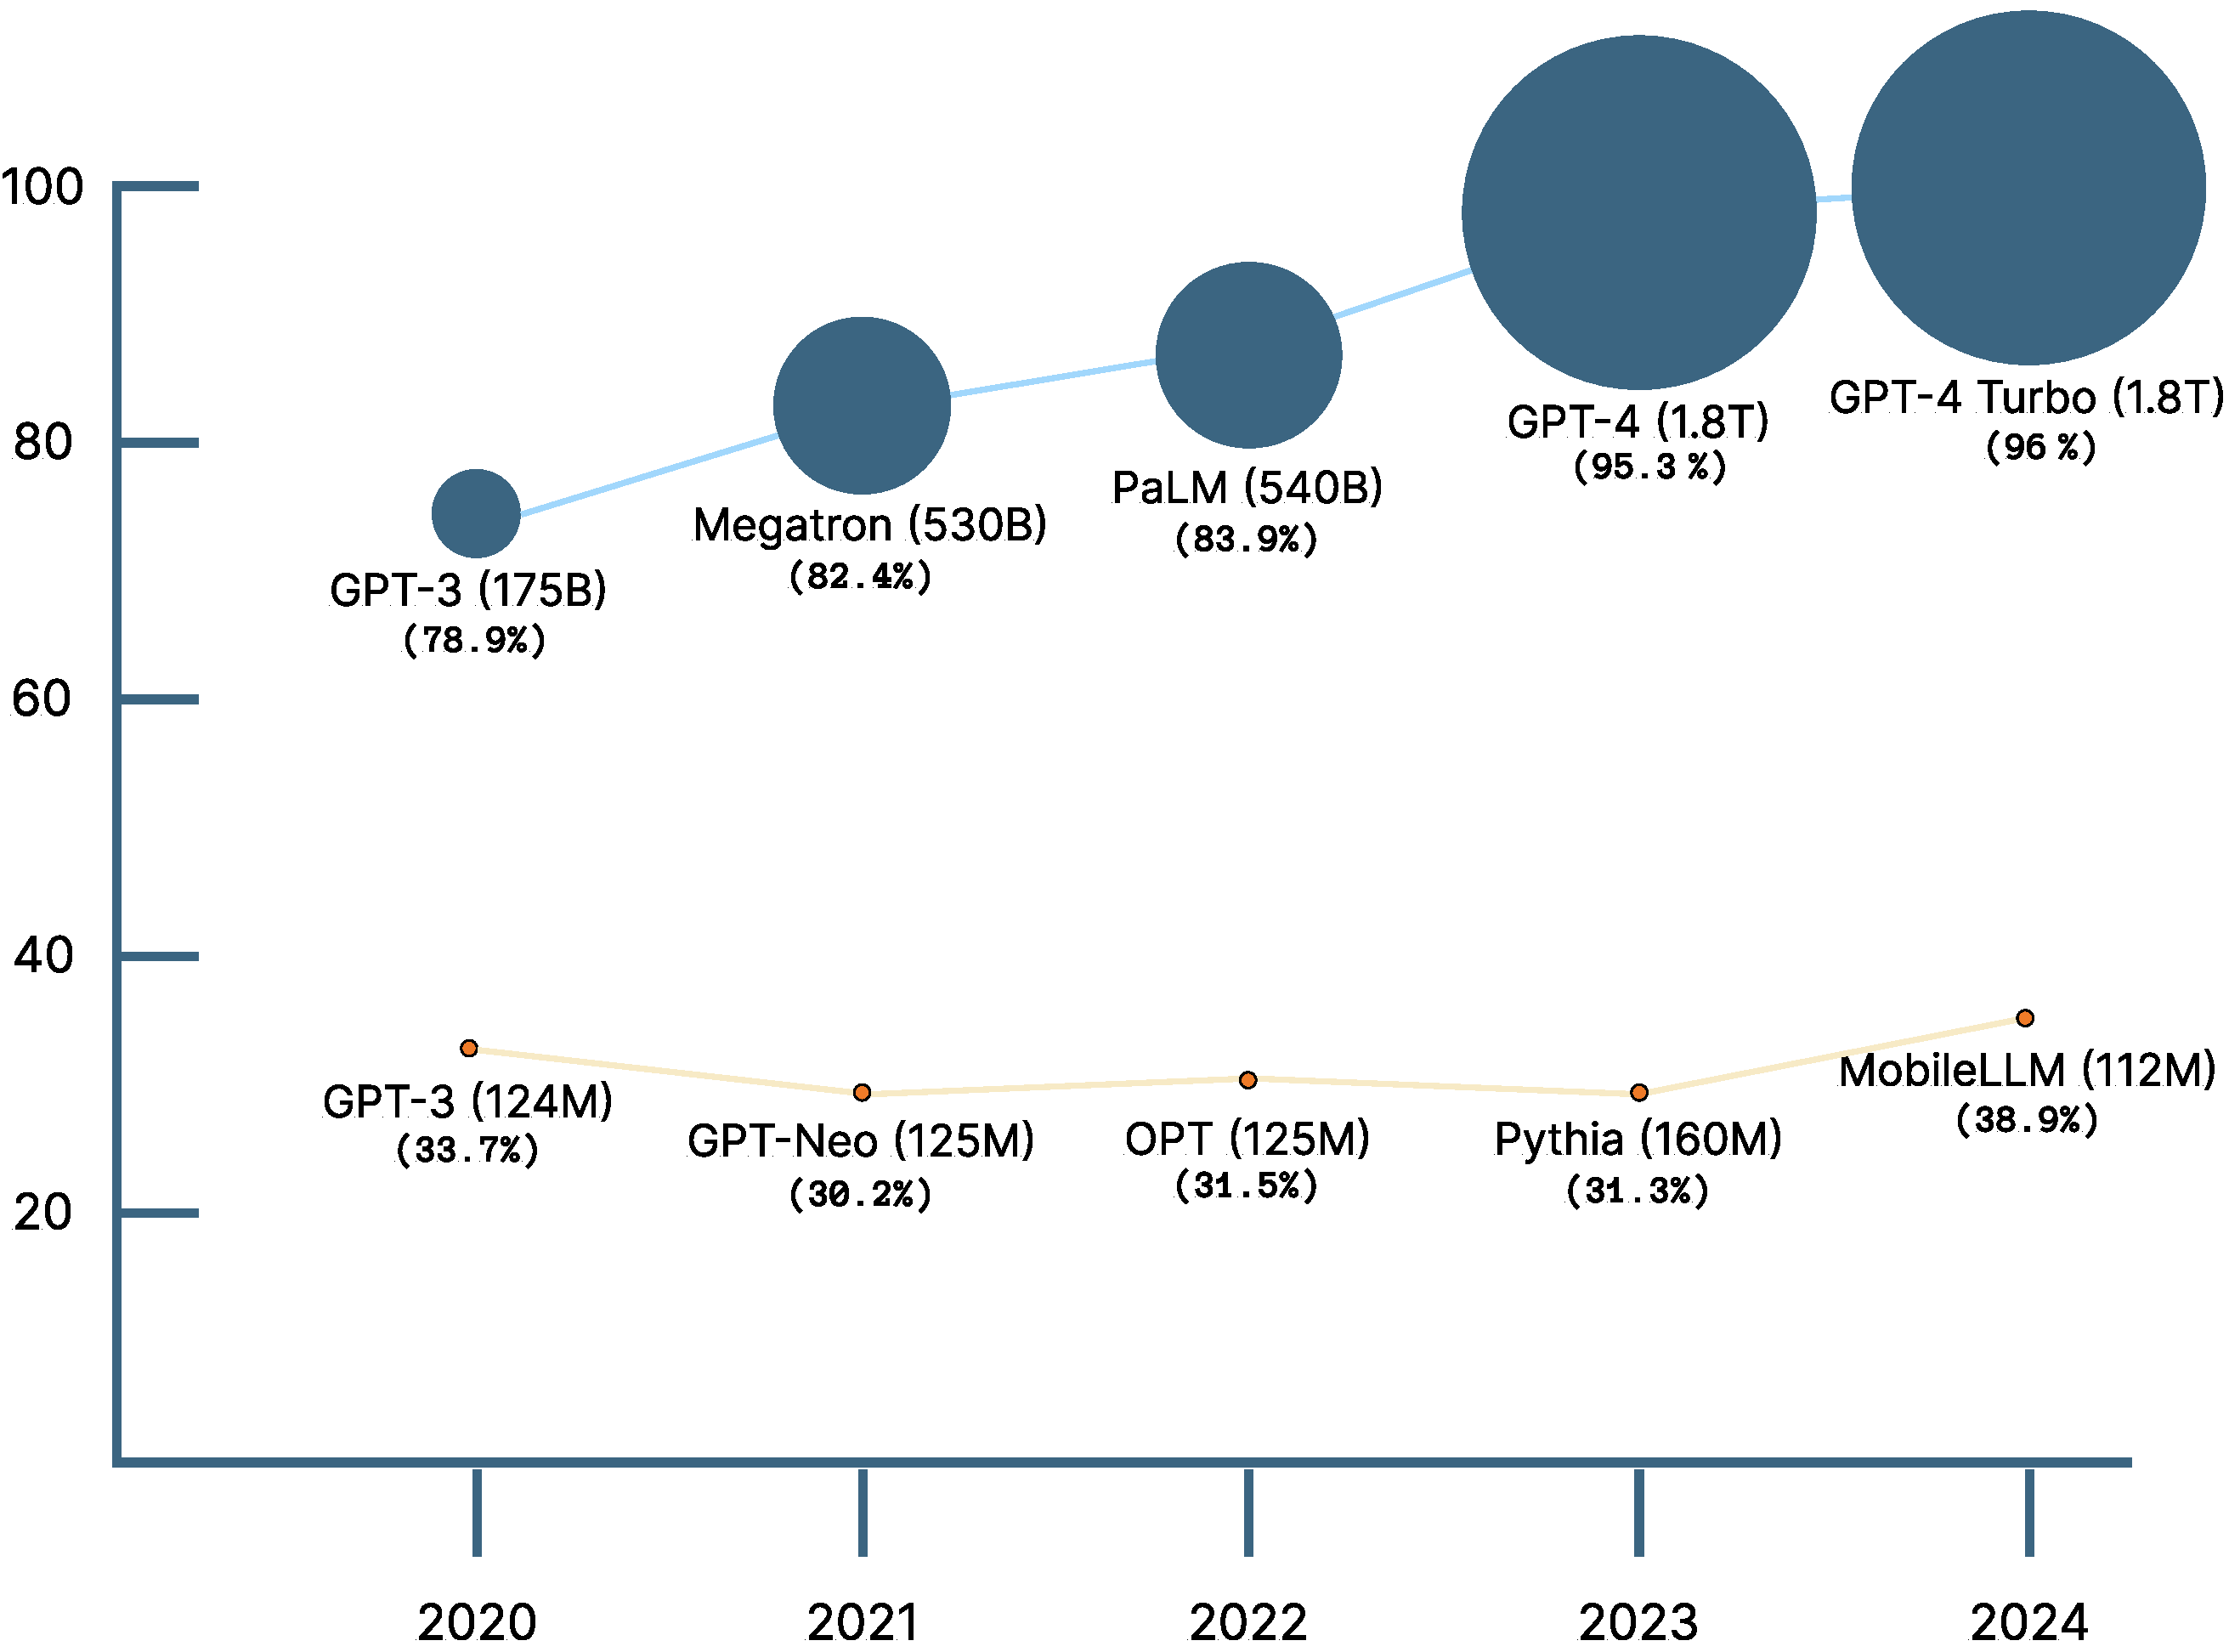
\includegraphics[width=0.8\textwidth]{chapters/introduction/figures/lm_performance_comparison.pdf}
    \caption{Performance of small and large language models on the HellaSwag dataset over time. The plot reveals a striking divergence: while \textbf{\textcolor[HTML]{37718E}{large}} models show consistent improvement, \textbf{\textcolor[HTML]{FF7F11}{small}} models of fixed size (e.g. 100M parameters) have plateaued despite advances in training techniques.}
    \label{fig:model_size_vs_performance}
\end{figure}

This insight extends beyond academic interest. While frontier models dominate public and industrial attention, small language models remain vital for several reasons. %They are not only essential for deployment in resource-constrained environments—such as mobile devices and edge computing—but also play a critical role in enabling transparency, reducing costs, and improving accessibility across a wider range of applications.

\section*{Why Do Small Models Matter?}

% We should also probably define what we mean by small models.

The rapid scaling of language models has brought about remarkable capabilities, but it has also surfaced a host of challenges and risks \citep{bommasani2021foundation}. Small language models, \textit{which I define as models with fewer than 1 Billion (1B) parameters}, offer a promising counterbalance. While the distinction between small and large models is relative to the scale being compared, the 1B parameter threshold provides a practical cutoff: a model with 1B parameters requires approximately 8GB of memory (assuming 32-bit precision) and can therefore be managed on a single GPU or deployed on-device with the hardware available as of 2025. Models of this scale offer several key benefits over their large counterparts:

\paragraph{Large models introduce significant societal risks.} As enumerated by the Stanford Center for Research on Foundation Models \citep{bommasani2021foundation}, these include the potential for generating disinformation and misinformation at scale, and amplifying biases and discrimination present in training data. The wide-spread adoption of these models across industries also raises concerns about the creation of single points of failure: a widely deployed model that is compromised could have cascading negative effects across all downstream applications. Relatedly, the authors highlight that these risks are not just technical but also social, as they can entrench power in the hands of a few organisations and make it harder to adapt models to specific or local needs.

\paragraph{Large models pose serious environmental sustainability challenges.} Researchers have increasingly emphasised energy efficiency as a core evaluation metric, on par with traditional measures like accuracy \citep{schwartz2020greenai}. Studies have quantified the financial and carbon costs of training state-of-the-art NLP systems, revealing orders-of-magnitude differences between large and small models \citep{strubell2019energy}. Tools like the ML Emissions Calculator \citep{lacoste2019quantifying} and systematic reviews of emissions factors \citep{luccioni2023counting} have made it clear that model size, hardware, and training recipes all play a role in determining the environmental footprint of machine learning. Transformer-based models \citep{vaswani2017attention}, in particular, are among the most energy-intensive, given their dense feed-forward architectures. Benchmarks such as HULK \citep{zhou2021hulk} have compared pretrained models' energy efficiency, showing that inducing sparsity and pruning models to reduce their size yields large environmental efficiency. Furthermore, the geographic location where models are trained can significantly affect emissions \citep{patterson2021carbon}; small models that can be trained locally remove the networking cost of distributed, remote model training and serving required by large models. 

%The overall trend is clear: smaller models are more sustainable, and their adoption is crucial for reducing AI's environmental impact.
% For example, a modest increase in translation accuracy can result in a dramatic rise in compute cost.

\paragraph{Data privacy and memorisation risks are heightened in large models.} Research has shown that neural networks, especially large ones, can memorise and regurgitate rare or sensitive training data \citep{feldman2020neural, carlini2019secret}. Follow-up studies have demonstrated that memorisation increases with model size and data duplication \citep{carlini2021extracting, carlini2022quantifying}; in particular, larger models are more likely to leak personally identifiable information, especially when trained on duplicated or low-diversity data \citep{huang2022large, neel2023privacy}. Recent so-called `scaling laws for memorisation' have quantified the relationship between model size and their propensity to memorise and leak sensitive information \citep{lu2024scaling, biderman2023emergent, kiyomaru2024comprehensive}. Mitigation strategies such as differential privacy \citep{dwork2006calibrating} and federated learning \citep{mcmahan2017communication} have been proposed, but these often come with trade-offs in model utility.% In contrast, smaller models by having less capacity to memorize and that can be managed locally offer a more privacy-preserving alternative—especially when combined with privacy-focused training techniques.
% TODO: Edit last sentence

\paragraph{Small models are uniquely suited for on-device and edge deployment.} Efficient inference with limited memory is essential for running language models on consumer hardware. Sub-billion parameter models are particularly important for energy-efficient, on-device applications, as demonstrated by \citet{liu2024mobilellm}. Early advances in mobile-friendly neural network architectures, such as MobileNets \citep{howard2017mobilenets} and EfficientFormer \citep{li2022efficientformer}, laid the groundwork for efficient models in both vision and language domains. More recently, research teams from cellphone manufacturers like Apple and Google have spear-headed efforts to optimise mobile-first models, with efforts to optimise the memory bandwidth of on-device language models \citep{alizadeh2024llm} and build custom hardware accelerators for serving models \citep{deepmind2023gemini}. %The importance of energy-proportional memory for datacenter and mobile applications has also been highlighted \citep{malladi2012towards}. 
 

\paragraph{Interpretability and scientific understanding are reasons to prioritise small models.} The internal mechanisms of transformers and other neural architectures are more tractable in smaller models, making them better testbeds for developing scientific understanding \citep{elhage2021mathematical, elhage2022toy, anthropic2023components}. Tools such as influence functions are easier to apply at small scale, and the ``manifold hypothesis" suggests that neural representations of language models (including those of larger models) often exist on a small manifold of the representational space \citep{olah2014manifolds}. More generally, as advocated for by \citet{elhage2021mathematical}, progress in understanding larger models often begins with insights gained from studying the structure of neural representations in smaller models.

\paragraph{The democratisation and accessibility of language technology depend on the availability of small, open models.} The cost of training and deploying large models is rising rapidly, with the financial and hardware requirements putting them out of reach for most organisations and individuals \citep{cottier2024rising, sharir2020cost}. Minimal, and small-scale implementations of language models like nanoGPT \citep{karpathy2023nanogpt} and Pico (introduced in Chapter 7) make language modelling accessible to a broader community, supporting experimentation, and innovation. By lowering the barrier to entry, small models enable more researchers to participate in the development and application of language technologies.

% In summary, small language models matter because they are more sustainable, privacy-preserving, interpretable, and accessible. They offer a practical and ethical path forward for language technology, especially as the risks and costs of large-scale models continue to mount.

\section*{Research Objectives}

This thesis aims to explore how small language models can be trained more efficiently and effectively using principled approaches, rather than brute-force scaling. The work is structured around two central research objectives:

\begin{quote}
    \textbf{Research Question 1 (RQ1): Can insights from human language acquisition be leveraged to develop more principled and effective training paradigms for small language models?}
\end{quote}

Despite recent advances in architecture design and model size compression techniques, small models continue to lag behind their larger counterparts. A persistent challenge is that many of the methods proposed to improve small models, ranging from ad hoc architectural tweaks to various forms of regularisation or data augmentation, often lack a strong scientific foundation. Progress is often marginal and difficult to interpret; new techniques sometimes offer only small gains or fail to generalise beyond specific benchmarks. Without a principled framework or guiding thesis, it becomes challenging to systematically understand what works, why it works, and how to build on prior results in a cumulative way.

One promising guiding thesis is to look to human language acquisition for inspiration. While today's large language models are trained on trillions of tokens, a typical 13-year-old human has been exposed to only around 100 million words \citep{warstadt2023babylm1}. This dramatic discrepancy highlights a key inefficiency in current training paradigms and suggests an opportunity: do strategies that work well for the human brain also confer advantages in artificial models? And can cognitive science offer a roadmap toward more efficient language modelling? 

Importantly, the aim of this work is not to model the mechanisms of human language acquisition per se. Humans and artificial networks learn in fundamentally different ways, and many aspects of human cognition remain poorly understood. Instead, I propose to use human learning only as a source of guiding hypotheses: where humans demonstrably exhibit effective learning behaviours (e.g., generalisation to novel words), it is valuable to test whether analogous strategies can benefit small language models.

By grounding small model training in insights from human cognition, this thesis seeks to move beyond ad hoc heuristics and toward a more principled, theory-driven foundation. The goal is to understand how cognitive strategies, such as curriculum learning, inductive biases, and compositional generalisation, translate into practical improvements in model design and training. In doing so, this work aims to bridge the gap between machine learning and cognitive science, offering not only empirical results but also conceptual tools for building small language models that are both efficient and robust.

To complement this exploration of training strategies, the second research objective focuses on understanding the learning dynamics of small models more deeply and rigorously.

\begin{quote}
    \textbf{Research Question 2 (RQ2): How can researchers more quantitatively understand how small models learn and how can this understanding be used to improve model design and training?}
\end{quote}

Improving training efficiency is only part of the broader challenge. Equally important is developing a deeper understanding of the underlying learning dynamics that drive how language models learn: How can we quantitatively study the learning process of language models? And how can we can we use these insights to improve model design and training? These questions demand not just better engineering, but a more scientific, principle-driven approach to model understanding.

In recent years, efforts to improve small language models have often relied on empirical heuristics that offer marginal gains. This trial-and-error mindset obscures the mechanisms behind success and makes it difficult to generalise progress across tasks or domains. To make progress, the research community must focus on the learning process itself: how knowledge is acquired, how model capacity is structured and used, and how different factors shape convergence dynamics. Small models provide a unique lens for this investigation not only because they are easier to analyse, but because their behaviour often reveals the underlying structure of learning in ways large models conceal.

By focusing on measurable, interpretable properties of training, such as model convergence dynamics and representational capacity, I hope to turn language model development into a more principled science. Furthermore, I aim to develop tools that enable the analysis and understanding of the learning dynamics of small models. These tools will support a more principled approach to model development, allowing researchers to systematically test training strategies and interventions instead of relying on trial-and-error. Building tools and frameworks that make the process of developing small models more scientific and accessible to a broader audience is a key goal of this thesis.
% This research objective, therefore, is grounded in the belief that meaningful progress in model development must be built on a deeper understanding of the learning process itself.
\section*{Thesis Overview}

This thesis is organised into two parts, reflecting the two research threads:

\subsection*{Part I: Cognitive Insights for Efficient Training (Chapters 2-–4)}

\begin{itemize}

    \item \textbf{Chapter 2:} \emph{Language Modelling: Foundations, Scale, and Efficiency} offers both an overview of the development and current state of language modelling, and a review of the major strategies for training language models more efficiently. The chapter first introduces foundational concepts in language modelling that are used throughout the thesis. I then review existing strategies for training language models more efficiently; from architectural innovations, optimisation techniques, and data calibration methods. I conclude by drawing connections between machine learning and cognitive science, considering how insights from human language acquisition can inform more principled model development, especially in resource-constrained environments.

    \item \textbf{Chapter 3:} \emph{Curriculum Learning for Infant-inspired Model Building: A Framework for Human-like Language Acquisition}  
    explores a systematic investigation of curriculum learning strategies inspired by human language acquisition, focusing on their application to small language models. The work is motivated by the striking data efficiency of human language learning compared to current language models.

    The chapter introduces \climb, a framework that operationalises three key aspects of human language acquisition into a curriculum learning framework: a vocabulary curriculum that gradually expands a model's lexicon, a data curriculum that orders training inputs by linguistic complexity and an objective curriculum that transitions from coarse word-class prediction to fine-grained masked language modelling.

    Using the BabyLM Challenge's strict 10-million-word training cap as a testbed, this work develops an optimised ``vanilla" BabyBERTa baseline that I use as a benchmark against the three curriculum learning approaches. The empirical results reveal that while individual curricula do not consistently outperform this baseline, they offer selective advantages when combined together and on specific linguistic tasks, particularly in syntactic evaluation.

    \item \textbf{Chapter 4:} \emph{Learning Words Like Humans Do: Syntactic Smoothing for Language Model Training}  
    explores how language models can learn word representations more like humans do, by leveraging syntactic structure to improve the representation of infrequent tokens. This work addresses a fundamental challenge in language modelling: while humans are able to leverage the linguistic structure of language to quickly learn new words, language models struggle to effectively represent tokens that appear rarely in their training data. This inefficiency stems from the maximum likelihood training objective, which disproportionately optimises frequent tokens while leaving infrequent ones with insufficient learning signals. In contrast to human language acquisition, language models learn frequency statistics that results in infrequent tokens being pushed into a narrow manifold of the representational space (a phenomenon known as `anisotropy'). 

    In this chapter, I show that this training process leads models to encode, what I term, a `frequency bias' and provide a mechanism for quantifying this bias. Next, inspired by how humans leverage syntactic knowledge to learn new words efficiently, I introduce \smoothing, a novel technique that improves token representations by incorporating linguistic structure into the learning process. By using part-of-speech distributions as a proxy for syntactic similarity, this method enables infrequent tokens to benefit from the learning signals of syntactically similar tokens. This approach mirrors the way humans use syntactic knowledge to learn new words efficiently and demonstrates how insights from human language acquisition can lead to more principled and effective training paradigms for language models.

\end{itemize}

\subsection*{Part II: An Analytical Lens on Learning Dynamics (Chapters 5--7)}

\begin{itemize}
    \item \textbf{Chapter 5:} \emph{Analysing Language Models: Foundations, Methods, and Tools} introduces the analytical foundations for studying the learning dynamics of language models. I present a range of complementary approaches for analysing these dynamics, including memorisation and data influence methods, representational convergence and similarity metrics, and capacity usage via sparsity, norm evolution, and rank-based analysis. These tools can be used to reveal how internal structures in language models develop, and how the learning trajectories of smaller models diverge from their larger counterparts.

    The chapter also situates this analysis within the broader interpretability literature, like attention pattern analysis, probing methods, and mechanistic interpretability. This background chapter lays the groundwork for the next two chapters, which apply these tools to understand and intervene in the learning dynamics of small language models.

    \item \textbf{Chapter 6:} \emph{Tending Towards Stability: Convergence Challenges in Small Language Models} examines why small language models often exhibit unstable or delayed convergence during training. I use the Pythia model suite to compare learning dynamics across model sizes, focusing on how internal layer activations evolve and how efficiently models use their representational capacity.

    I apply Centered Kernel Alignment (CKA) to track the convergence of activations over time and introduce Proportional Effective Rank (PER) as a new metric to assess how layers utilise their parameters and gradients. My findings show that larger models converge more quickly and consistently, while smaller models underutilise capacity, leading to erratic learning and premature saturation.
    
    These results suggest that small models suffer from inefficient learning trajectories, not just limited capacity. The chapter closes by identifying the need for an intervention-friendly training framework to test hypotheses about improving small model training which motivates the design of the \pico framework presented in Chapter 7.

    \item \textbf{Chapter 7:} \emph{\pico: A Lightweight Framework for Studying Language Model Learning Dynamics} introduces \pico, a modular framework designed to support the scientific development of language models.

    \pico consists of two core components:
    
    \begin{enumerate}
        \item \texttt{pico-train}, a minimalist training library that logs model weights, activations, and gradients at regular intervals, and
        
        \item \texttt{pico-analyze}, a companion toolkit that computes metrics such as PER, CKA, sparsity, and norm dynamics across layers and checkpoints.
    \end{enumerate}

    Together, these tools enable researchers to systematically explore how architectural or training interventions affect learning dynamics. A typical workflow involves formulating a hypothesis, implementing the corresponding modification in \texttt{pico-train}, and using \texttt{pico-analyze} to evaluate its effects. This creates a feedback loop for iterative, and systematic model development. This chapter presents several case studies to illustrate how \pico supports this process in practice.

\end{itemize}

\section*{Contributions}

This thesis makes the following contributions to the study of small language models:

\vspace{1em}

\textbf{1. Cognitively inspired training strategies for small language models}

\begin{itemize}

    \item Presents \climb, a three-pronged curriculum learning framework based on principles from human language acquisition. \climb both defines and operationalises three forms of curriculum learning that operate on the vocabulary, input data, and objective function. While these strategies are intuitively appealing, I find that they offer limited benefit in practice, making \climb a comprehensive and critical evaluation of human-inspired curricula for language model training (Chapter 3).

    \item Proposes \smoothing, a cognitively motivated method that mimics how humans use grammatical structure to infer the meaning of rare words. By diffusing learning signals across syntactically similar tokens, the approach reduces frequency bias and improves representation of low-frequency words (Chapter 4).

\end{itemize}

\textbf{2. A quantitative framework for analyzing learning dynamics in small models}

\begin{itemize}
    \item Introduces a set of metrics for quantifying both how effectively layers in a language model use their representational capacity over time and how well a model converges to a stable representation (Chapter 6).

    \item Applies these metrics to show that small models converge more slowly and inconsistently than larger models due to inefficient internal capacity usage.

\end{itemize}

\textbf{3. An open-source platform for training-time analysis and reproducible experimentation}
\begin{itemize}
    \item Presents \textbf{\pico}, a modular framework for developing language models in a scientific, hypothesis-driven way. \pico integrates two libraries that enable researchers to iteratively train and analyse language models in a systematic and reproducible way (Chapter 7).

    \item Releases the \textbf{\pico Model Suite}, a family of small- to mid-sized models (11M–-570M parameters) trained with standardised recipes and full checkpoint access that can be used as a starting point for scaling studies, and interpretability research.
\end{itemize}

\newpage
\section*{Publications}

The content of this thesis is comprised of the following published conference papers and software packages.

\begin{tcolorbox}[
    enhanced,
    colback=white,
    colframe=thesisblue,
    arc=0mm,
    boxrule=1pt,
    left=10pt,
    right=10pt,
    top=10pt,
    bottom=10pt,
    title=Published Works,
    fonttitle=\bfseries,
    coltitle=white
]
\subsection*{Thesis Publications}
The following papers and software packages form the core content of this thesis.

\begin{itemize}
    \item Richard Diehl Martinez, Zebulon Goriely, Hope McGovern, Christoper Davis, Andrew Caines, Paula Buttery, Lisa Beinborn (2023). {\color{thesisblue}\href{https://aclanthology.org/2023.conll-1.10/}{CLIMB – Curriculum Learning for Infant-inspired Model Building}}. In \emph{Proceedings of the BabyLM Challenge at the 27th Conference on Computational Natural Language Learning}, pages 138--154, Singapore. Association for Computational Linguistics.

    \item Richard Diehl Martinez, Zebulon Goriely, Andrew Caines, Paula Butery, Lisa Beinborn (2024). {\color{thesisblue}\href{https://aclanthology.org/2024.emnlp-main.486/}{Mitigating Frequency Bias and Anisotropy in Language Model Pre-Training with Syntactic Smoothing}}. In \emph{Proceedings of the 2024 Conference on Empirical Methods in Natural Language Processing}, pages 8541--8565, Miami, Florida, USA. Association for Computational Linguistics.

    \item Richard Diehl Martinez, Pietro Lesci, Paula Buttery (2024). {\color{thesisblue}\href{https://aclanthology.org/2024.findings-emnlp.246/}{Tending Towards Stability: Convergence Challenges in Small Language Models}}. In \emph{Findings of the Association for Computational Linguistics: EMNLP 2024}, pages 4253--4263, Miami, Florida, USA. Association for Computational Linguistics.

    \item Richard Diehl Martinez, David Demitri Africa, Yuval Weiss, Suchir Salhan, Ryan Daniels, Paula Buttery (2025). {\color{thesisblue}\href{https://github.com/pico-lm}{Pico: A Modular Framework for Hypothesis-Driven Small Language Model Research}}. Accepted to \emph{2025 Conference on Empirical Methods in Natural Language Processing System Demonstration Track}.
\end{itemize}
\end{tcolorbox}

\newpage

\begin{tcolorbox}[
    enhanced,
    colback=white,
    colframe=thesisblue,
    arc=0mm,
    boxrule=1pt,
    left=10pt,
    right=10pt,
    top=10pt,
    bottom=10pt,
    title=Additional Works,
    fonttitle=\bfseries,
    coltitle=white
]
\subsection*{Mentored Works}
I mentored the following projects during my PhD.

\begin{itemize}
    % \item David Demitri Africa, Yuval Weiss, Paula Buttery, Richard Diehl Martinez (2025). {\color{thesisblue}{Learning Dynamics of Meta-Learning in Small Model Pretraining}}. In Submission to \emph{BlackBox Workshop at the 2025 Conference on Empirical Methods in Natural Language Processing}.
    \item Yuval Weiss, David Demitri Africa,  Paula Buttery, Richard Diehl Martinez (2025). {\color{thesisblue}{Investigating ReLoRA: Effects on the Learning Dynamics of Small Language Models}}. Accepted to \emph{BlackBox Workshop at the 2025 Conference on Empirical Methods in Natural Language Processing}.
    \item David Demitri Africa, Yuval Weiss, Paula Buttery, Richard Diehl Martinez (2025). {\color{thesisblue}{Filipino Zero-Shot Transfer Using Meta-Pretraining for Named Entity Recognition}}. In Submission to \emph{Multilingual Representation Learning Workshop at the 2025 Conference on Empirical Methods in Natural Language Processing}.
\end{itemize}

\subsection*{Other Publications}
I also worked on the following papers during my PhD (not included in this thesis).

\begin{itemize}
    \item Cole Simmons, Richard Diehl Martinez, Dan Jurafsky (2024). {\color{thesisblue}\href{https://aclanthology.org/2024.ml4al-1.20/}{SumTablets: A Transliteration Dataset of Sumerian Tablets}}. In \emph{Proceedings of the 1st Workshop on Machine Learning for Ancient Languages}, pages 192-202, Bangkok, Thailand. Association for Computational Linguistics.
    \item Zebulon Goriely, Richard Diehl Martinez, Andrew Caines, Paula Buttery, Lisa Beinborn (2024). {\color{thesisblue}\href{https://aclanthology.org/2024.conll-babylm.4/}{From Babble to Words: Pre-Training Language Models on Continuous Streams of Phonemes}}, In \emph{Proceedings of the BabyLM Challenge at the 27th Conference on Computational Natural Language Learning}, pages 37--53, Miami, Florida, USA. Association for Computational Linguistics.
    \item Suchir Salhan, Richard Diehl Martinez, Zebulon Goriely, Paula Buttery (2024). {\color{thesisblue}\href{https://aclanthology.org/2024.conll-babylm.15/}{Less is More: Pre-Training Cross-Lingual Small-Scale Language Models with Cognitively-Plausible Curriculum Learning Strategies}}, In \emph{Proceedings of the BabyLM Challenge at the 27th Conference on Computational Natural Language Learning}, pages 174--188, Miami, Florida, USA. Association for Computational Linguistics.
    \item  Richard Diehl Martinez$^{\dagger}$, Suchir Salhan$^{\dagger}$, Zebulon Goriely, Paula Buttery (2025). {\color{thesisblue}{How Long Can a \textsc{BabyLM} Go? Investigating the Effect of Sequence Length on Small Language Model Pre-Training}}. Accepted to \emph{2025 BabyLM Workshop at the Conference on Empirical Methods in Natural Language Processing}. $^{\dagger}$Equal contribution.
\end{itemize}
\end{tcolorbox}